\chapter{Integration Engineering}
\label{sec:fdsp-coord-integ-sysengr}
%\chapter{Integration}
%\label{vl:tc-integration}

%[Farshid/Terri]

The focus of the integration engineering is the mechanical and
electrical configuration and interfaces between each of the detector
systems. This includes verification that subassemblies and their
interfaces are correct (e.g., \dword{apa} and \single \dword{pds}). A
second major area is in the support of the \dwords{detmodule} and
their interfaces to the cryostat and cryogenics. A third major area is
assuring that the \dwords{detmodule} can be installed --- that the
integrated components can be moved into their final configuration. A
fourth major area is in the integration of the \dwords{detmodule} with
the necessary services provided by the conventional facilities.


The \dword{tc} engineering team will maintain configuration data in
the appropriate format for the management of the detector
configuration. The consortia provide engineering data for their
subsystems to \dword{tc}. The \dword{tc} engineering team will work
with the \dword{lbnf} project team to integrate the full detector data
into the global \dword{lbnf} configuration files.

These tasks are carried out utilizing tools and practices
described in the rest of this chapter.

\section{Integration Models}
\label{sec:fdsp-coord-integ-models}
The single phase and dual phase detectors are large and made from many
intricate components. Fortunately, and for the most part, the
components are repetitive and are not overly complex geometrically. As
such, 3D mechanical modelling techniques are well suited for
representation of the detectors and management of its configuration.


At the same time, 3D modelling techniques are varied in the way items
are represented and in the way the techniques are practiced. This
requires that a set of 2D integration drawings are generated which are
clear and unambiguous across the collaboration. Such 2D drawings form
the basis of the 3D models and the basis of engineering design of all
components.

\subsection{Static Models}
\label{sec:fdsp-coord-integ-static}
Technical coordination is responsible for generating and maintaining
the 3D detector integration models and generating and maintaining the
2D integration drawings. These models are static as they represent all
components at their design dimension. They do not represent effects of
gravity, tolerances, cold temperature and installation and assembly
clearances.

The 3D models are assembled by combining component models from various
consortia. The 3D model files are shared with the consortia in a
read-only fashion. The 2D integration drawings are then generated and
disseminated which show the interfaces to the level of detail that is
necessary to ensure proper fit and function. Issues that arise are
communicated with the consortia and resolution method is
determined. It is important to note that \dword{tc} engineering team
will not make any changes to any of the consortia component models.

It is the responsibility of the consortia to resolve any issues per
agreed method and provide updated models for reintegration. As such
models are kept in synchronization with only one-way integration and
without modification by anyone other than the consortia.

The level of detail in a model is managed actively as inordinate
levels of detail lead to large file sizes when models are combined and
then incorporated into global models of facilities. It is the
responsibility of the \dword{tc} engineering team to ensure the
appropriate level of detail is incorporated at each stage of model
integration.

Figure~\ref{fig:dune-sp_overall} shows the overall model of the Single Phase Detector.
\begin{dunefigure}[Overall model of the Single-Phase Detector]{fig:dune-sp_overall}
  {Overall model of the Single-Phase Detector.}
%  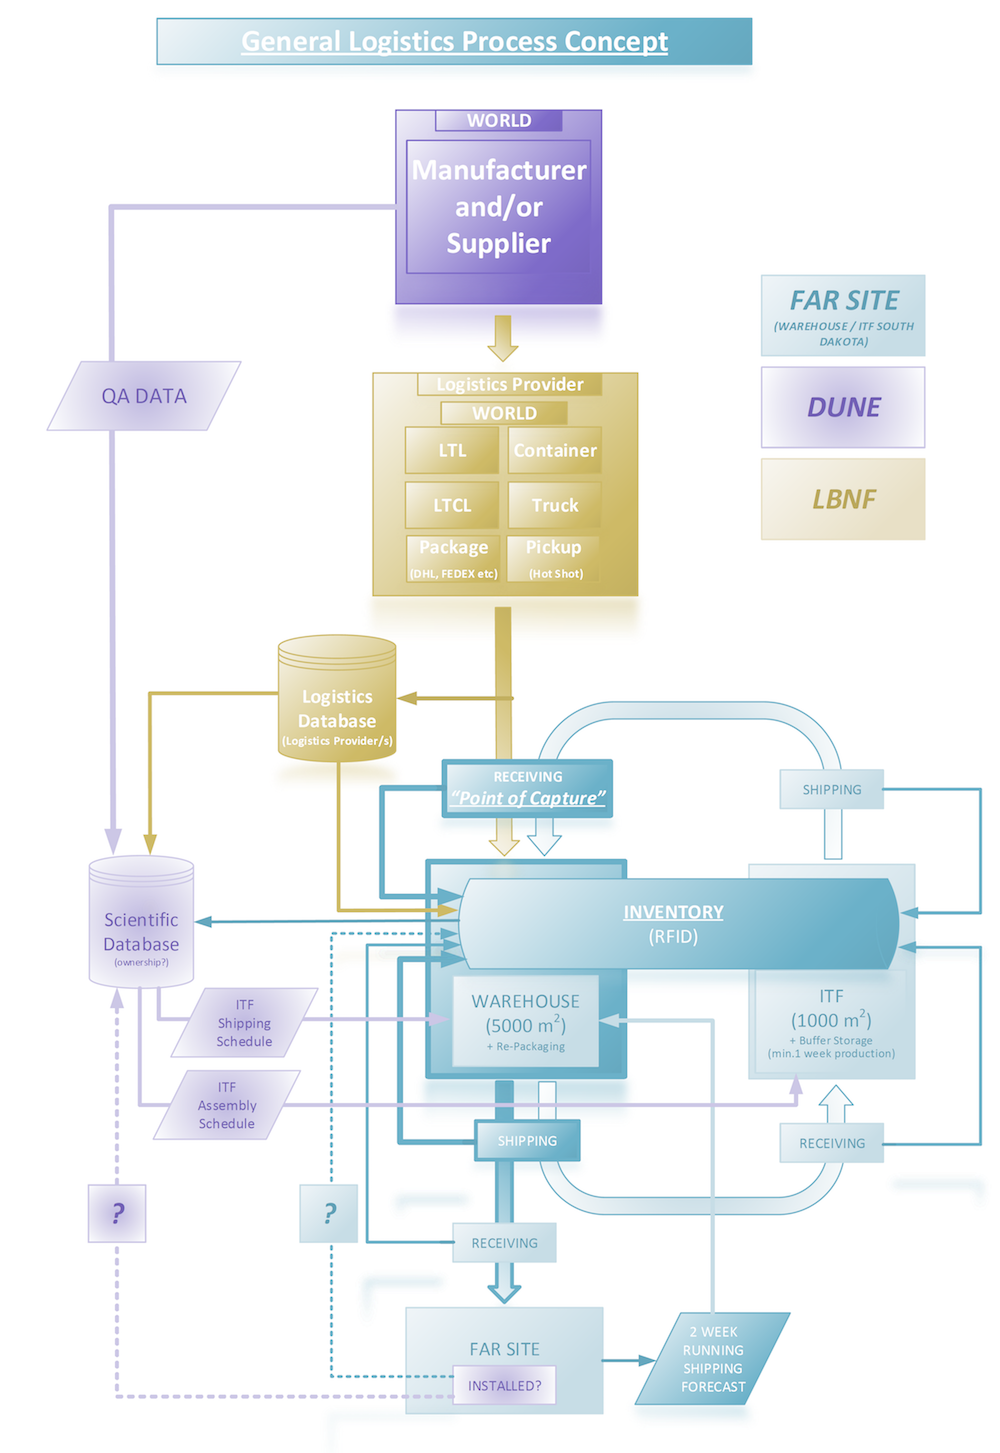
\includegraphics[width=0.85\textwidth]{logistics.png}
\end{dunefigure}
One wall of the cryostat is removed for the interior components to be
visible. The detector is made from 25 rows. Which are the same in
construction. At the end of row one and row 25, end walls are
installed which close the detection volume.

As mentioned earlier, this model does not include all the details of
the detector components. The components are simplified to keep the
overall model complexity to a manageable level.

Figure~\ref{fig:dune-sp_row} shows the model of one row of the
detector module.
\begin{dunefigure}[Overall model of one row of the Single-Phase Detector]{fig:dune-sp_row}
  {Model of one row of the Single-Phase Detector.}
  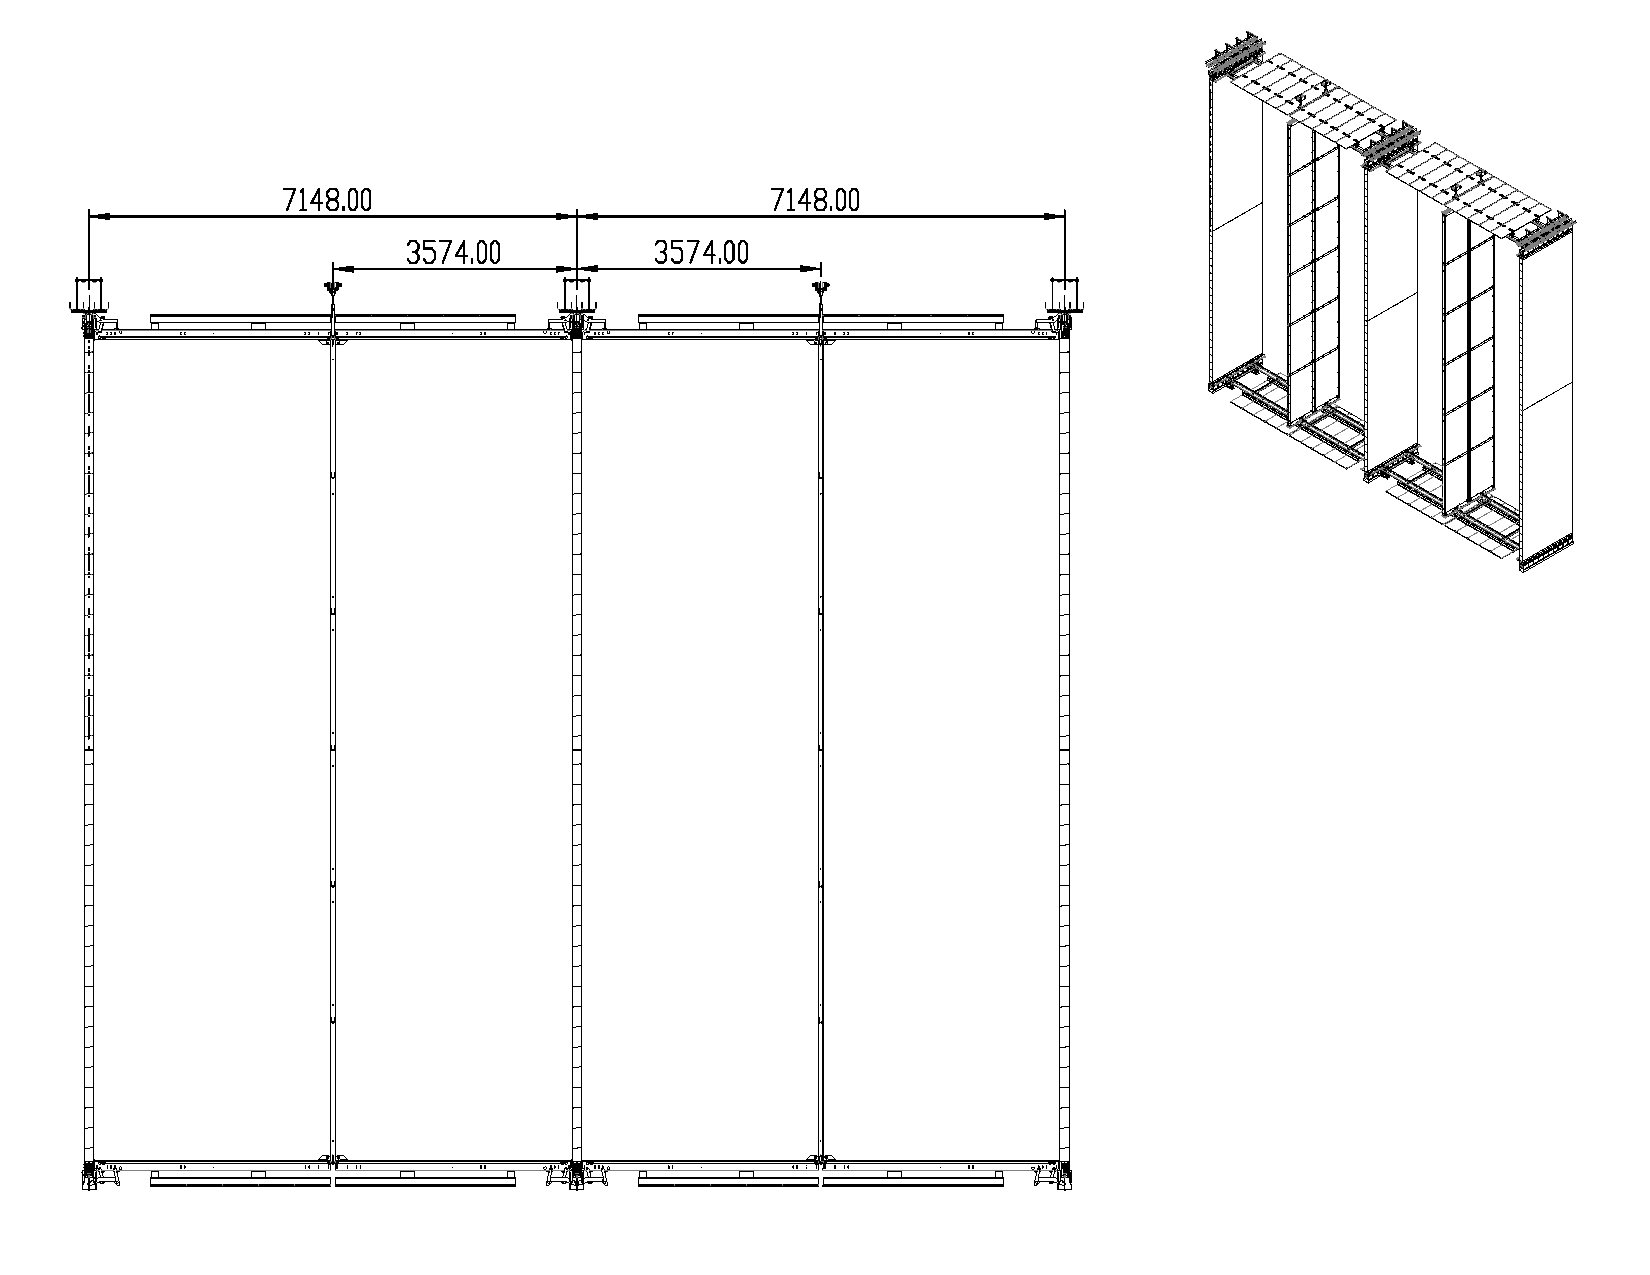
\includegraphics[width=0.6\textwidth]{Model_OneRow_SP.pdf}
\end{dunefigure}
Each row is made from six Anode Plane Assemblies,
four Cathode Plane Assemblies and eight Filed Cage plus Ground Plane
Assemblies. A total of 25 rows comprise one DUNE-SP far detector.

Figure~\ref{fig:dune-sp_transverse} and~\ref{fig:dune-sp_long} show
the cross sections of the detector in the transverse and longitudinal
directions respectively. Overall dimensions are also shown.
\begin{dunefigure}[Section view of the Single Phase Detector in the transverse direction.]{fig:dune-sp_transverse}
  {Section view of the Single Phase Detector in the transverse direction.}
  %  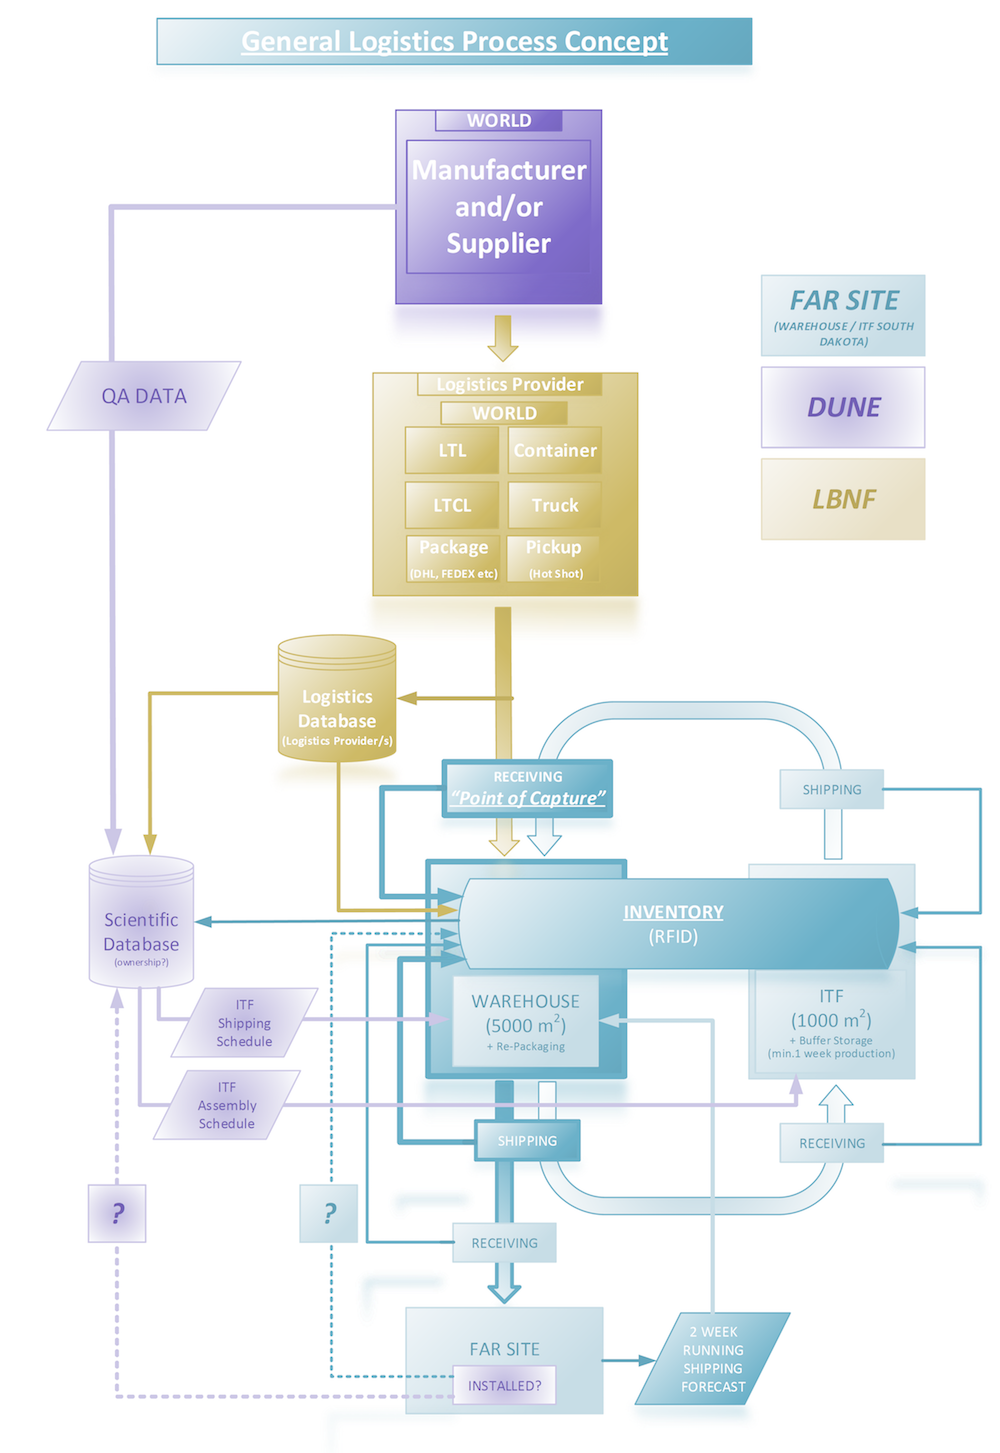
\includegraphics[width=0.85\textwidth]{logistics.png}
\end{dunefigure}
\begin{dunefigure}[Overall model of the Single Phase Detector in the longitudinal direction]{fig:dune-sp_long}
  {Overall model of the Single Phase Detector in the longitudinal direction.}
  %  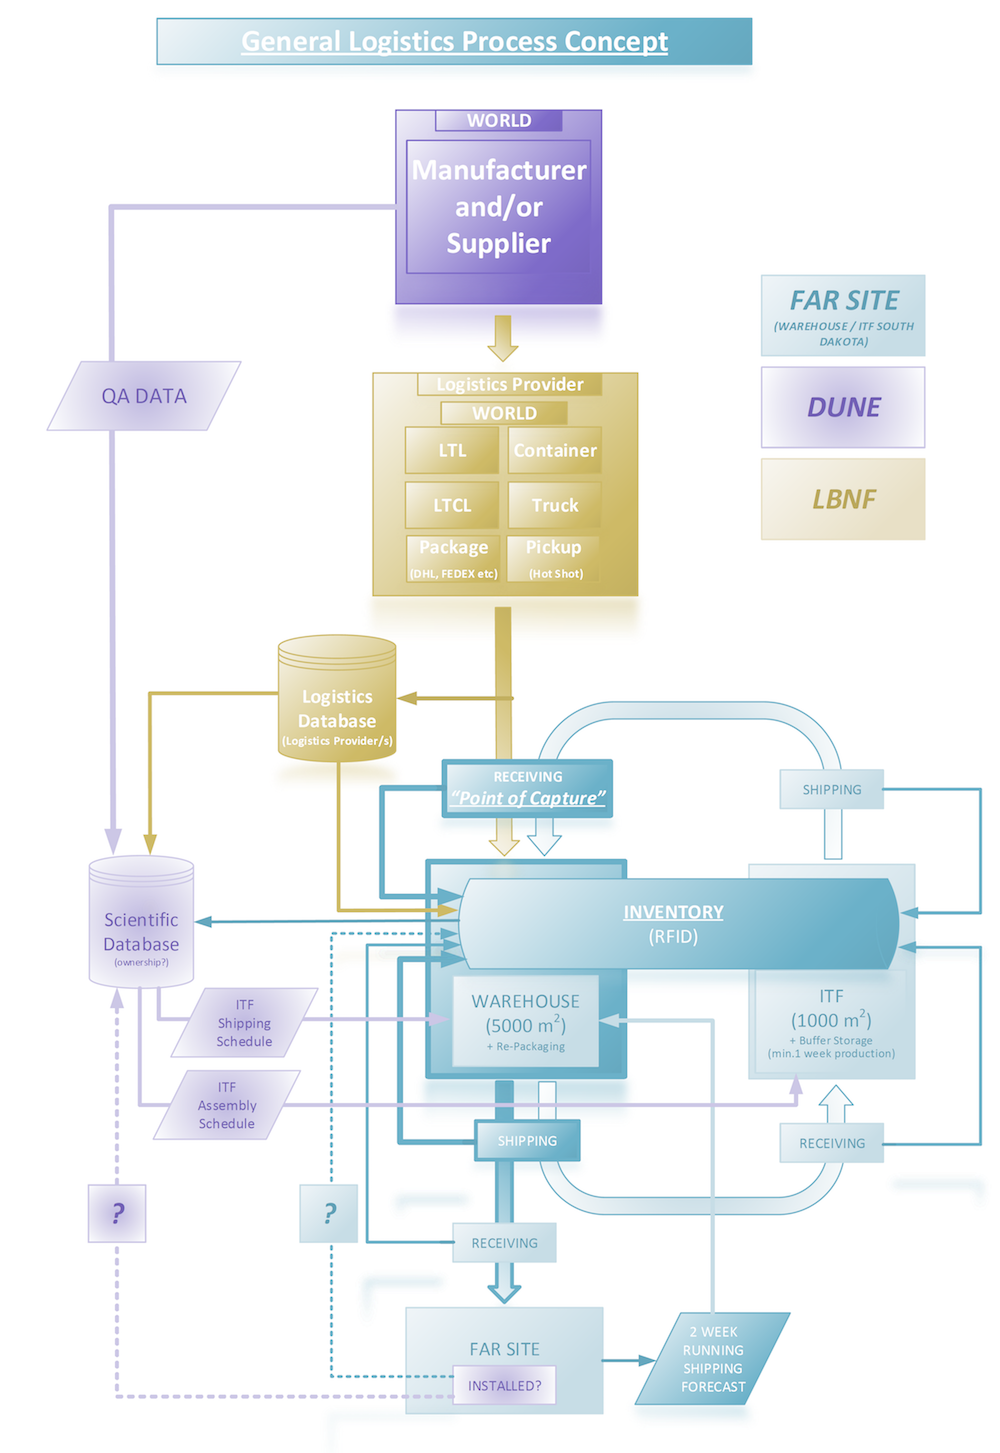
\includegraphics[width=0.85\textwidth]{logistics.png}
\end{dunefigure}

(Note: Need analogous figures and explanations for Dual Phase)

\subsection{Envelope and Assembly Models}
\label{sec:fdsp-coord-integ-envelope}
Static models represent the detector and its components at their
design dimension exactly. Such exact dimensions are needed for the
detail component drawings and model to be completely compatible at all
times.

For installation and operation, other envelope models are needed which
will be more approximate in nature. Envelope models will be developed
to account for issues that impact installation and operation:
\begin{enumerate}
 \item Effects on the detector caused by distortion of the cryostat
   and detector support structure due to gravity,
 \item Effects on the detector caused by thermal contraction during
   detector filling and operation,
 \item Overall envelope models due to effects of component and
   assembly tolerances,
 \item Clearances needed during installation and envelopes needed for
   access and tooling,
 \item Reference models and drawings needed for installation stages
   and for control of assembly,
 \item Reference models and drawings needed for alignment and survey.
\end{enumerate}


The models and drawings described above will be generated from static
models. Combination models of above will also be generated to
represent combined effects. In all case, as with static modes, 2D
drawings will be created which form the basis of the installation
drawings.

Generation of envelope models and drawings are the responsibility of
\dword{tc} engineering team in coordination with consortia.


\section{Plan for Model and Drawing Storage and Dissemination}
\label{sec:fdsp-coord-integ-modelplan}
Drawings, models, schematics, production data and all other
engineering documents are created and shared by consortia and by
\dword{tc} engineering team. In addition, all interface drawings and
documentation are generated by \dword{tc} engineering team and shared
in a similar fashion.

Folders have been set up that allow for uploading and sharing
documents with appropriate protection. The structure of the folders
has been setup in a way that will suit each consortium. Not all
consortia will have similar folder structures or files and will adapt
the structure to their needs.

The folders and files reside on the engineering data management system
(EDMS). This system and similar structures have been used for
ProtoDUNE and are being used by LBNF.

The following shows a high-level outline of the folder structure. The
first section is for technical coordination files. The following
section is generic and is for a consortium. There will be one such
folder for each consortium.
\begin{enumerate}
 \item Technical Coordination
 \begin{enumerate}
  \item Mechanical drawings and files (Control by F. Feyzi)
  \begin{enumerate}
    \item Far Detector general drawings for illustration purposes (control by TC)
    \item 3-D Model files of internal detector, for periodic upload to global model
    \item 2-D Interface drawing files    
    \item Alignment and survey files
    \item Integration Test facility
    \item Ash River installation test Technical Coordination
    \item QA/QC files
    \item Safety analysis and documentation
    \item Design reviews
  \end{enumerate}
  \item Electrical and Electronics(Control by T. Shaw)
  \begin{enumerate}
    \item Infrastructure Requirements for Grounding
    \item Consortia interface drawings
    \item Detector Electronics Grounding Guidelines
    \item Detector Safety System
    \item QA/QC files
    \item Safety analysis and documentation
  \end{enumerate}
 \end{enumerate}
 \item Consortia files (x10) (Control by consortia technical leads)
 \begin{enumerate}
   \item 3-D Model files
   \item 2-D Part drawing files
   \item Production files
   \item General Grounding Diagram
   \item System Level Block Diagram(s)
   \item System Level Wiring Diagram
   \item Software/Firmware Plans
   \item Custom Components (xN) if applicable (such as ASICs)
   \item PCB Component (xN)
   \item Cable Component (xN)
   \item Power Supply Component (xN)
  \end{enumerate}
\end{enumerate}
(Note: add figure once the EDMS structure is set up)



\section{Integration Drawings}
\label{sec:fdsp-coord-integ-drawings}
Within the detector, components from various consortia are assembled
and installed. The interfaces among components are developed and
managed through models and drawings as described earlier.

There are many such interfaces that are controlled. The following
section shows some of the interfaces, controlling dimensions and
configuration.

Figure~\ref{fig:dune-apa_interfaces_top} shows the interfaces for the top of the APAs.
\begin{dunefigure}[Interface between upper Anode Plane Assembly, Field Cage, cable trays and Detector Support System]{fig:dune-apa_interfaces_top}
  {Interface between upper Anode Plane Assembly, Field Cage, cable trays and Detector Support System.}
%  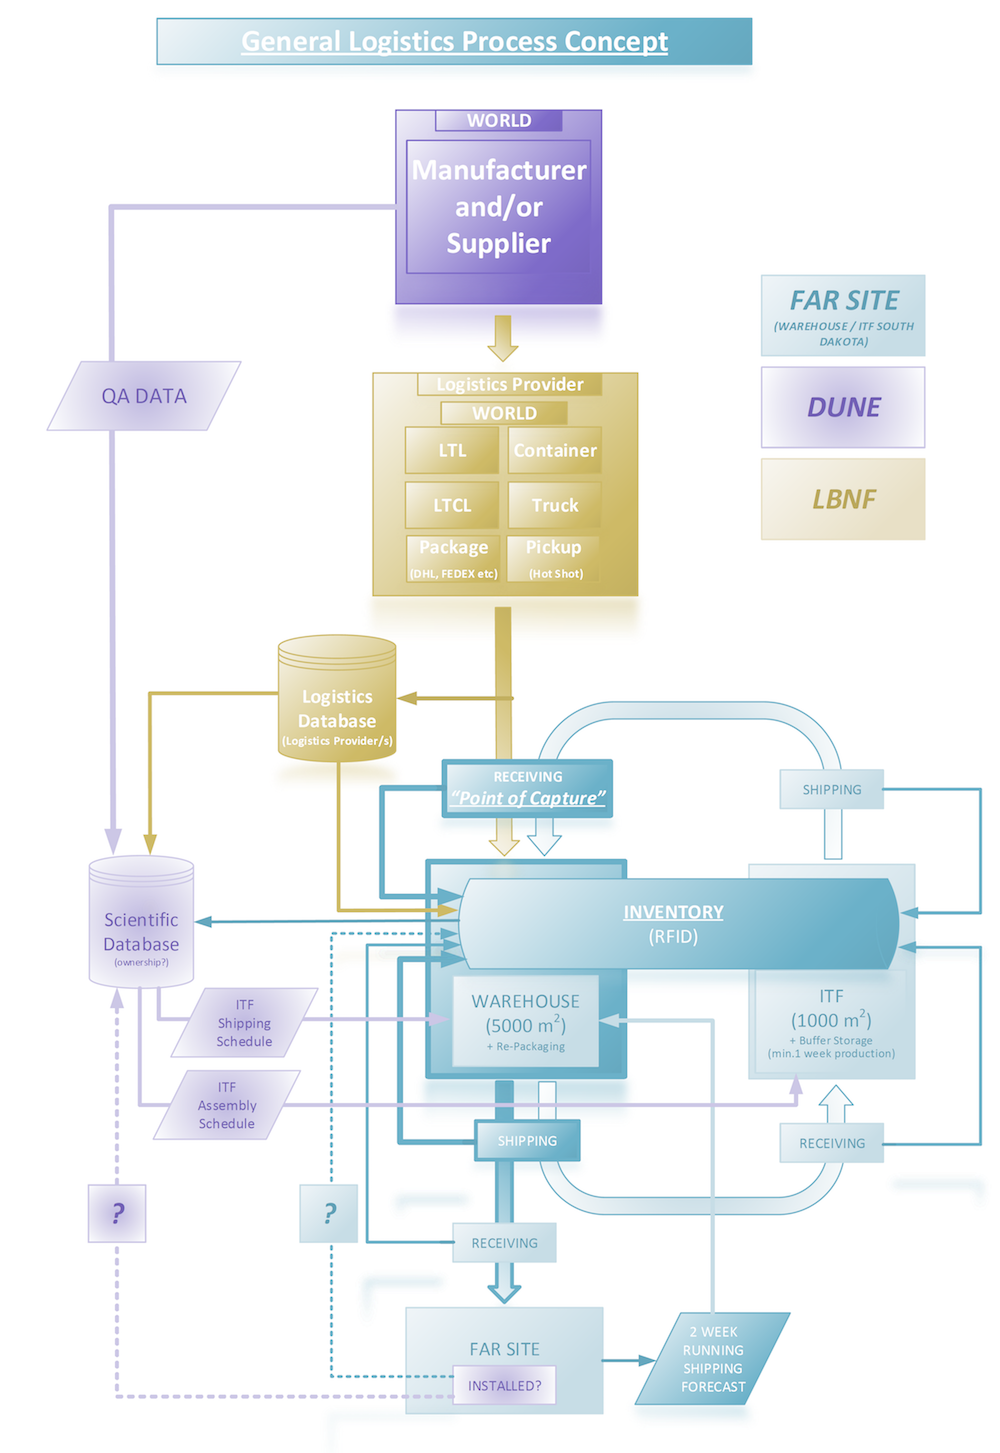
\includegraphics[width=0.85\textwidth]{logistics.png}
\end{dunefigure}

Fig~\ref{fig:dune-apa_interfaces_bottom} shows the interfaces for the bottom of the APAs.
\begin{dunefigure}[Interface between upper Anode Plane Assembly, Field Cage and service floor]{fig:dune-apa_interfaces_bottom}
  {Interface between upper Anode Plane Assembly, Field Cage and service floor.}
%  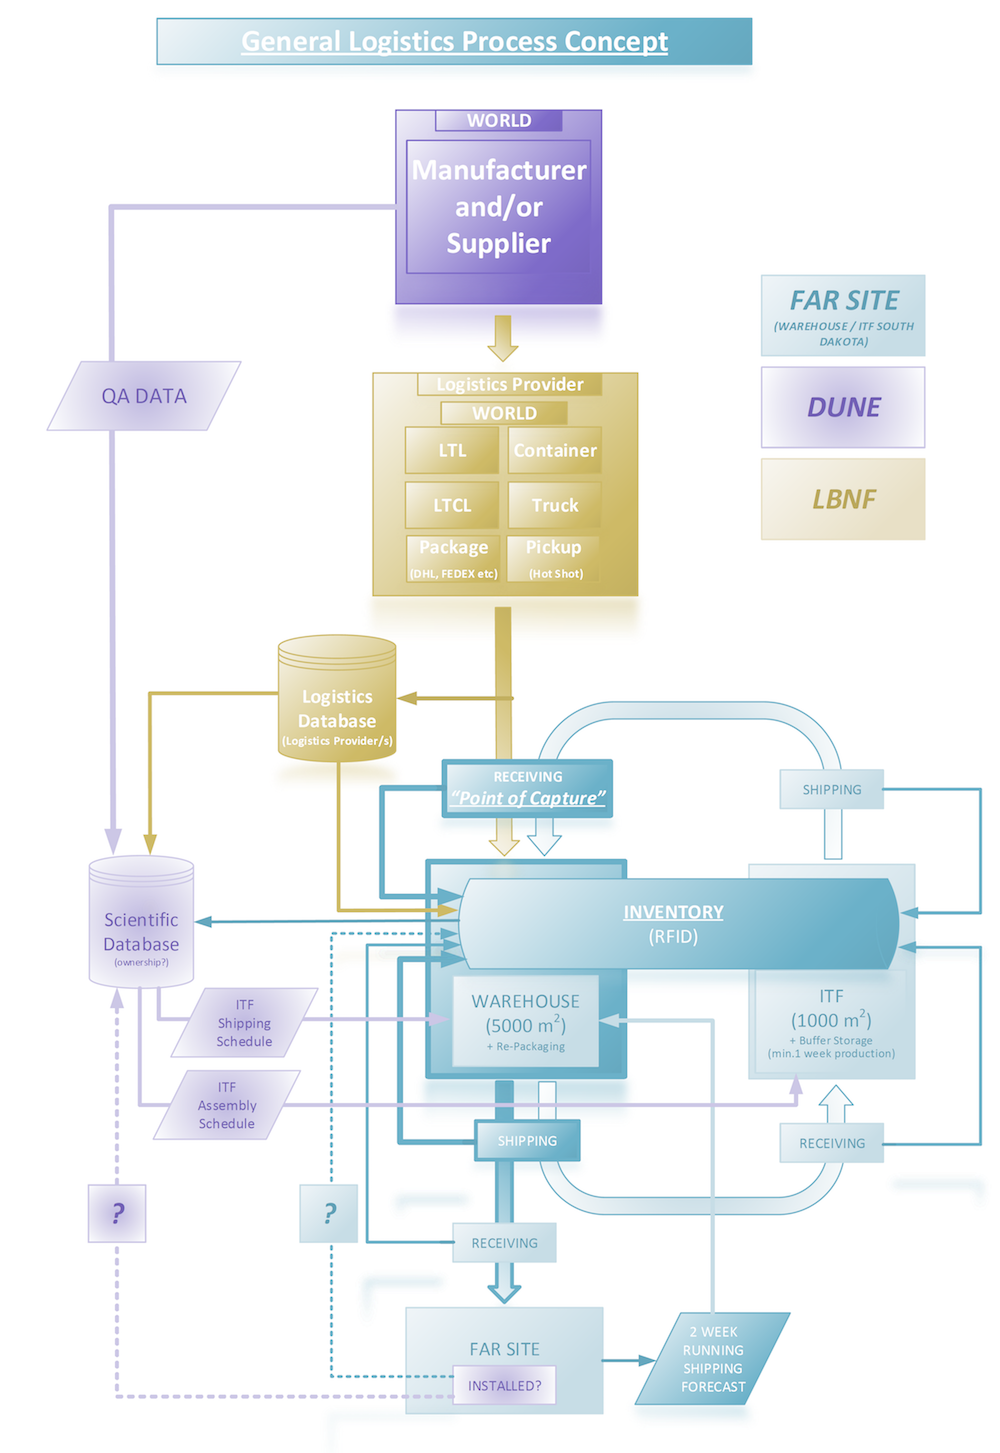
\includegraphics[width=0.85\textwidth]{logistics.png}
\end{dunefigure}

Fig~\ref{fig:dune-apa_interfaces} shows the interfaces for the top of the APAs and field cages.
\begin{dunefigure}[Interface between Cathode Plane Assembly, upper Field Cages and Ground Plane]{fig:dune-apa_interfaces}
  {Interface between Cathode Plane Assembly, upper Field Cages and Ground Plane.}
%  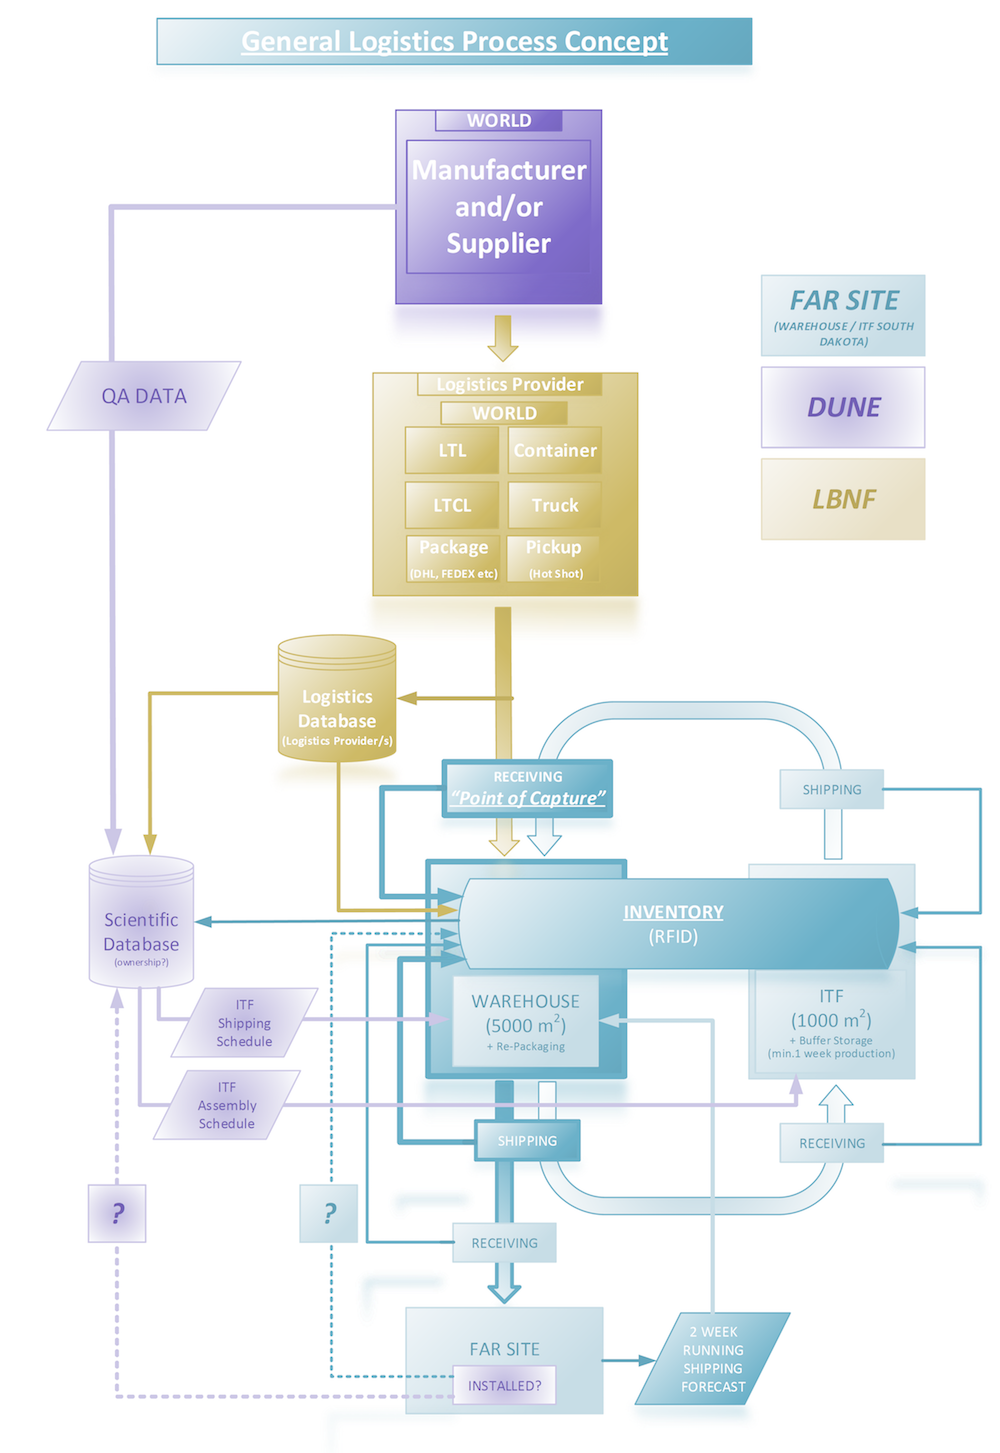
\includegraphics[width=0.85\textwidth]{logistics.png}
\end{dunefigure}

Component tolerances and installation clearances are managed through
additional models as described
earlier. Fig~\ref{fig:dune-apa_interfaces_top} is a graphical
representation of Anode Plane and Cathode Plane Assemblies. It also
shows them relieve position which defines how they are constrained in
the models. As such, component tolerances and installation clearances
do not affect the relative position in the warm state.

Fig~\ref{fig:dune-apa_envelope} shows the envelope for the APAs and field cages.
\begin{dunefigure}[Graphical representation of envelope dimensions and
    installation clearances for Anode Plane and Cathode Plane
    Assemblies in the warm state]{fig:dune-apa_envelope} {Graphical
    representation of envelope dimensions and installation clearances
    for Anode Plane and Cathode Plane Assemblies in the warm state.}
%  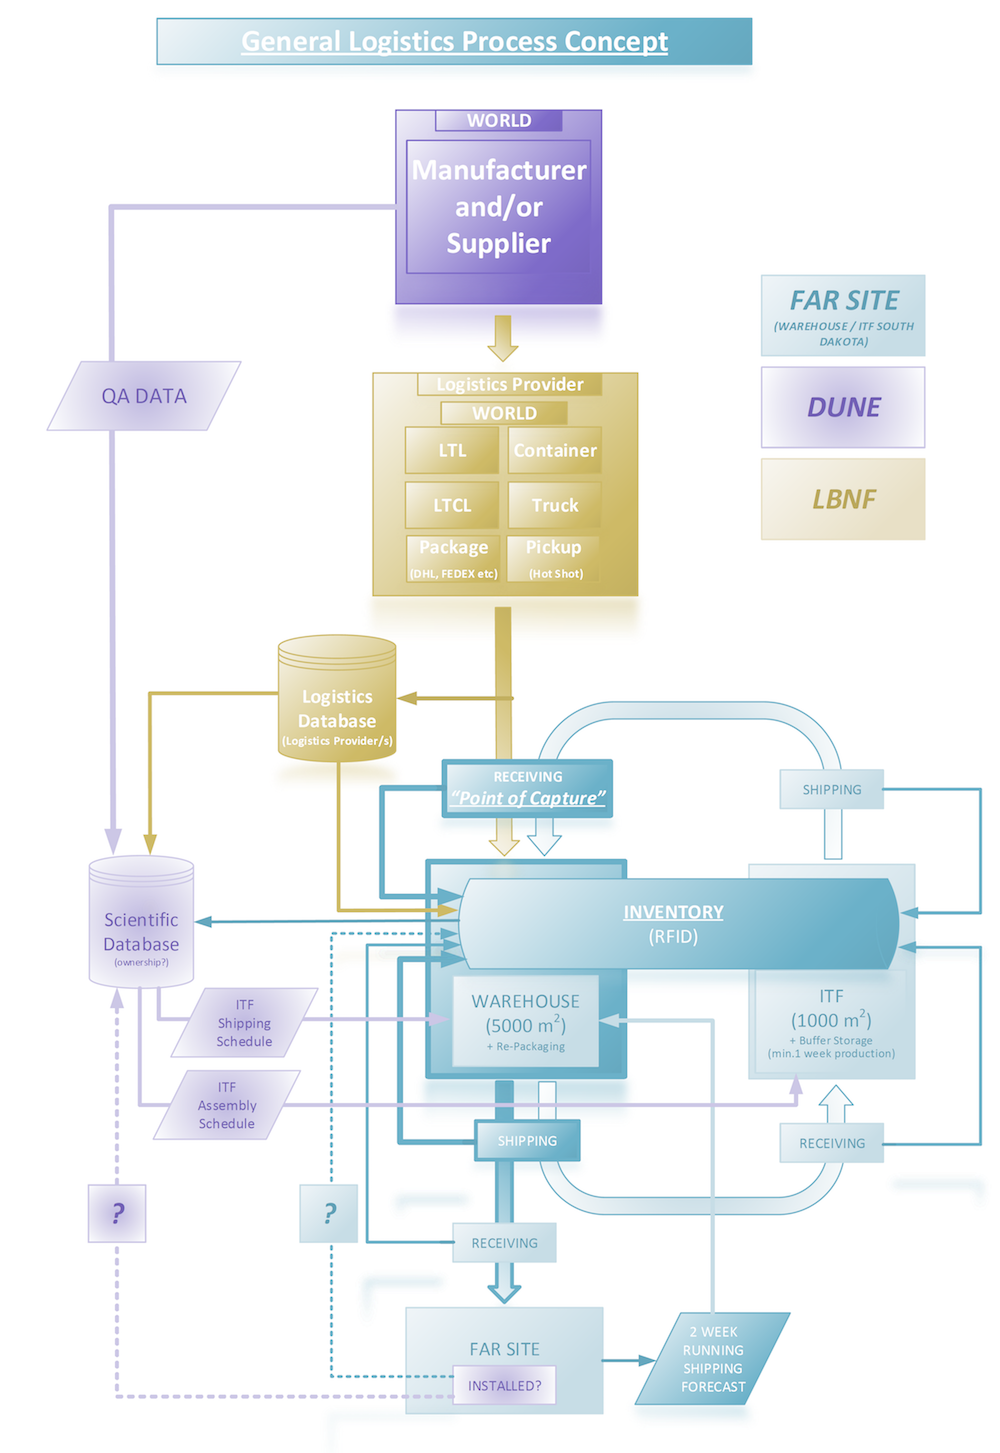
\includegraphics[width=0.85\textwidth]{logistics.png}
\end{dunefigure}


In the cold state, the relative position of groups of Anode Plane and
Cathode Plane Assemblies change due to thermal contraction, while
relative positions within each group are relatively
constant. Fig~\ref{fig:dune-apa_envelope_cold} is a graphical
representation in the cold state.
\begin{dunefigure}[Graphical representation of envelope dimensions and
    installation clearances for Anode Plane and Cathode Plane
    Assemblies in the cold state]{fig:dune-apa_envelope_cold} {Graphical
    representation of envelope dimensions and installation clearances
    for Anode Plane and Cathode Plane Assemblies in the cold state.}
%  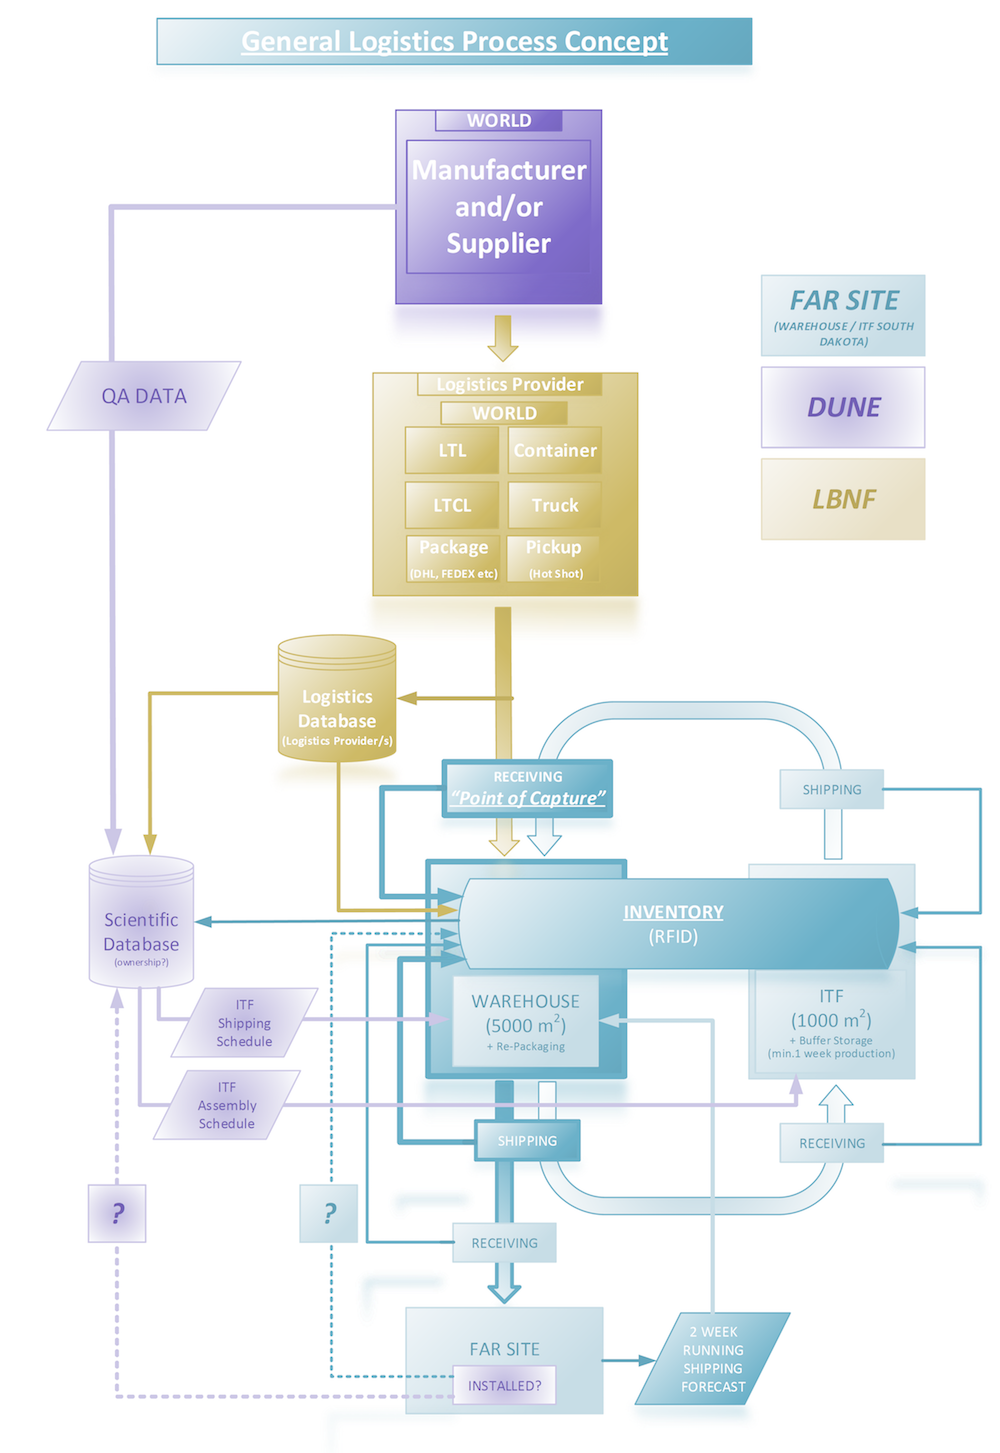
\includegraphics[width=0.85\textwidth]{logistics.png}
\end{dunefigure}

It should be noted that the design of the detector support system and
the cryostat have direct impact on the cold state. In addition,
effects of gravity and buoyancy are also not represented. Such effects
are under study and will be represented in the models as design
progress.

Prior to installation of the detector, a set of cryogenic distribution
pipes are installed on the floor of the cryostat. In addition, the
membrane of the cryostat will have corrugations that impede
movement. Therefore, a temporary service floor will be installed. The
floor will be installed, and later removed, in section. Fig shows this
interface.

Fig~\ref{fig:dune-floorpipes} shows the interface of cryogenic
distribution pipes, service floor and detector.
\begin{dunefigure}[Interface of cryogenic distribution pipes, service floor and detector.]{fig:dune-floorpipes} {Interface of cryogenic distribution pipes, service floor and detector.}
%  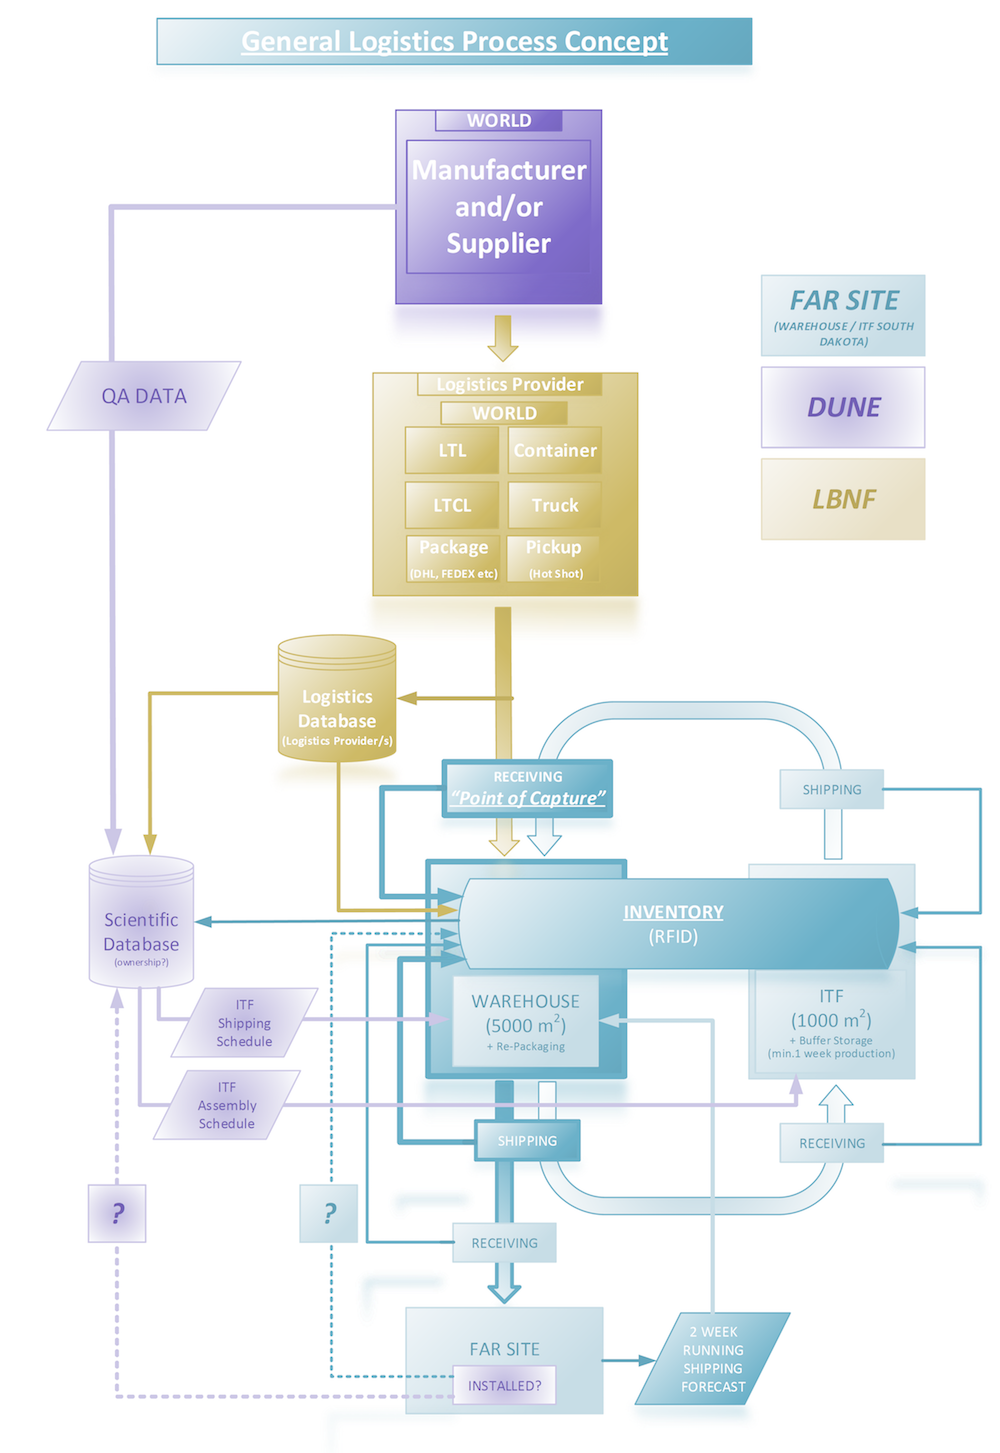
\includegraphics[width=0.85\textwidth]{logistics.png}
\end{dunefigure}


(Note: Need analogous figures and explanation for Dual Phase)


\section{Electrical System Block Drawings, Schematics, Layouts and Wiring Diagrams}
\label{sec:fdsp-coord-electrical}
%[Terri]


The electrical design aspects of each consortia can be described by a
set of documents which in all cases includes a system level block
diagram and one-line power/grounding documentation.  Furthermore,
depending on what is being described, a complete set of schematics,
board production files and wiring diagrams will be required.  All
designs are subject to an electrical safety review prior to
installation and the safety review process should be begun though
technical coordination early in the design process.

A system level block diagram must be produced by all consortia.  In
some cases, multiple system level block diagrams may be required.  An
example of this is for the Slow Controls Consortia, where multiple
types of systems (RTD readouts, Purity Monitors, Cameras, Pressure
sensors, etc.) will each require a separate system level block
diagram. A system level block diagram should show the conceptual
blocks required to be implemented in the design along with connections
to other conceptual block elements both within and outside of the
consortia.  An example of a system level block diagram can be found in
Figure~\ref{fig:electrical_blockdiagram_example}.
\begin{dunefigure}[Example system level block diagram]{fig:electrical_blockdiagram_example}
  {Electrical system level block diagram.}
  %  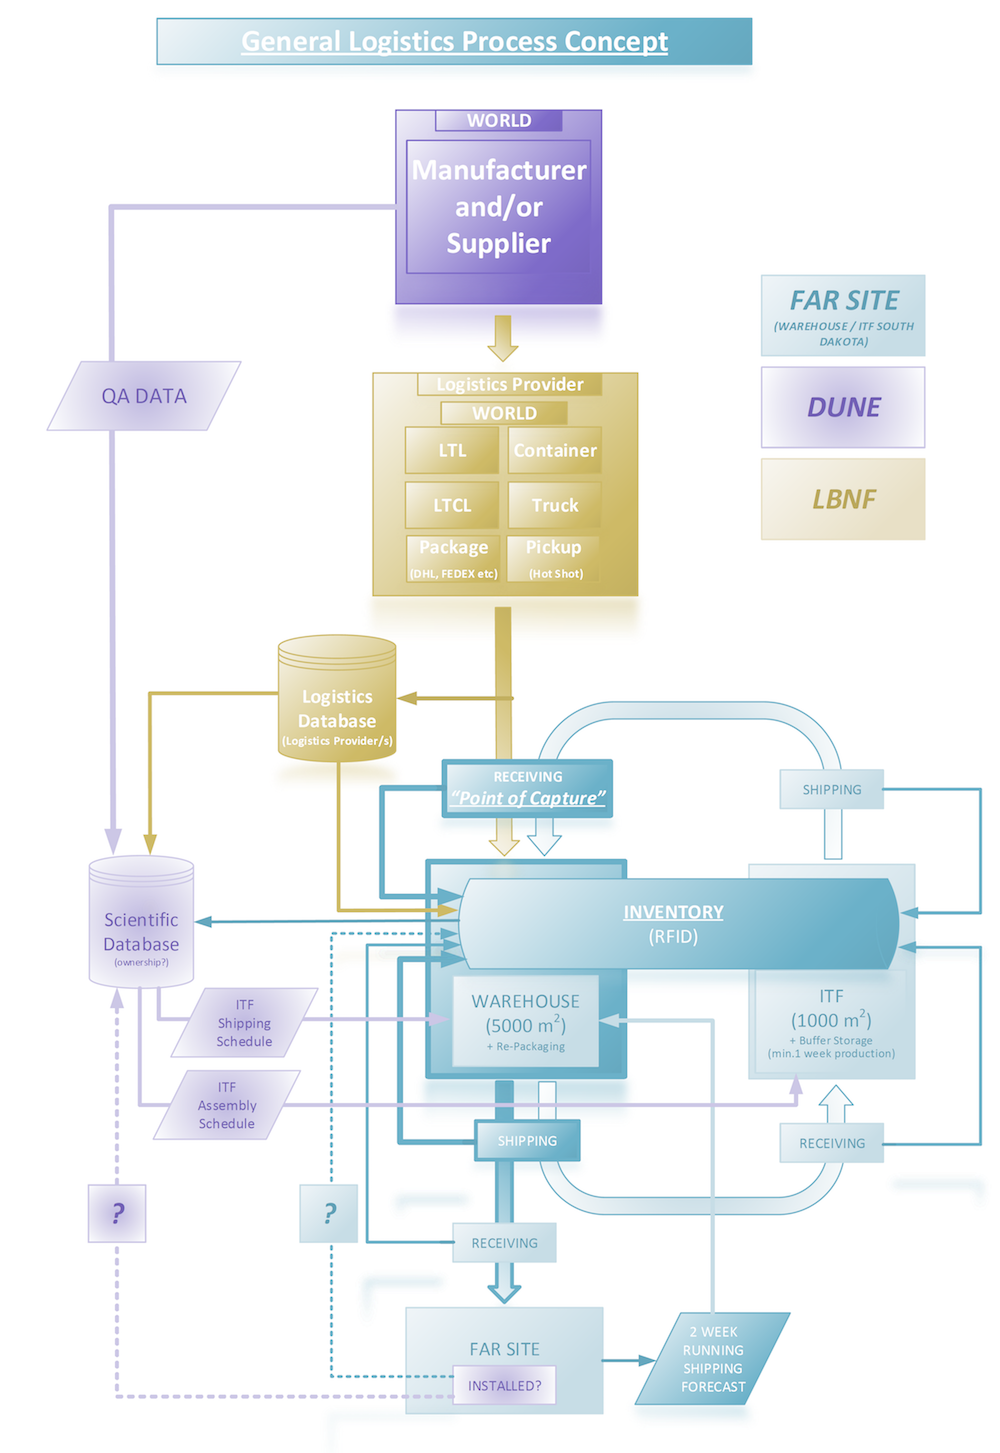
\includegraphics[width=0.85\textwidth]{logistics.png}
\end{dunefigure}

An electrical one-line drawing should represent the power and ground
distribution within the system being described.  The path of power and
ground distribution wiring between circuit elements should be
specifically noted along with wire types and sizes.  Power elements,
such as power supplies, fuses (or other protective circuit elements),
power connectors and pin ampacity should all be documented.

Electrical schematics show very specific details of how individual
components are connected.  Usually a schematic will represent a
printed circuit board design.  Schematics should call out specific
parts which are used in the design and include all interconnections.
In the case of a printed circuit board, layout files, manufacturing
specifications and bills of materials are also required to document
the design and allow for a safety review of any custom boards or
modules.

Wiring diagrams should include all wire and cable connections which
run between printed circuit boards or electronics modules.  Wires and
cables should be described within the contents of the diagram and
include identification of wire AWG, wire color, cable specification
and cable connectors and pinouts.


\section{Electrical Integration Drawings}
\label{sec:fdsp-coord-integ-electrical}
showing interfaces between subsystems... [Terri]


\section{Detector Survey and Alignment}
\label{sec:fdsp-coord-integ-survey}
The detector placement within the cryostat and thereby within the
cavern does not have a physics requirement. The requirement is driven
by the need for overall mechanical assembly in order that interfacing
parts are assembled and function properly.

In this section, reference frames for the detector are defined in order
that overall survey and alignment can be carried out with respect to
the cavern reference frame. (Note: we have not yet defined this)

For the single-phase detector, a reference flat and level plane is
defined which is coplanar with the upper Anode Plane Assembly yoke
planes. As such 75 yoke planes will define this reference flat and
level plane. This reference plane is set at exactly 781 mm below the
theoretical plane of the cryostat top membrane.

The detector reference plane is chosen to be coplanar with the upper
Anode Plane Assembly yoke planes because all the features of the
Plane, including the active area, are referenced to this plane.  Once
this plane is defined and established through survey, all vertical
distances within the detector are referenced and established to this
plane.  Fig~\ref{fig:detector_reference_plane} shows the reference
plane in relation to the cryostat top membrane, Anode Plane Assembly
active area, and detector Support Syste
\begin{dunefigure}[Reference plane relative to the cryostat, Anode Plane Assembly and Detector Support System]{fig:detector_reference_plane}
  {Reference plane relative to the cryostat, Anode Plane Assembly and Detector Support System.}
%  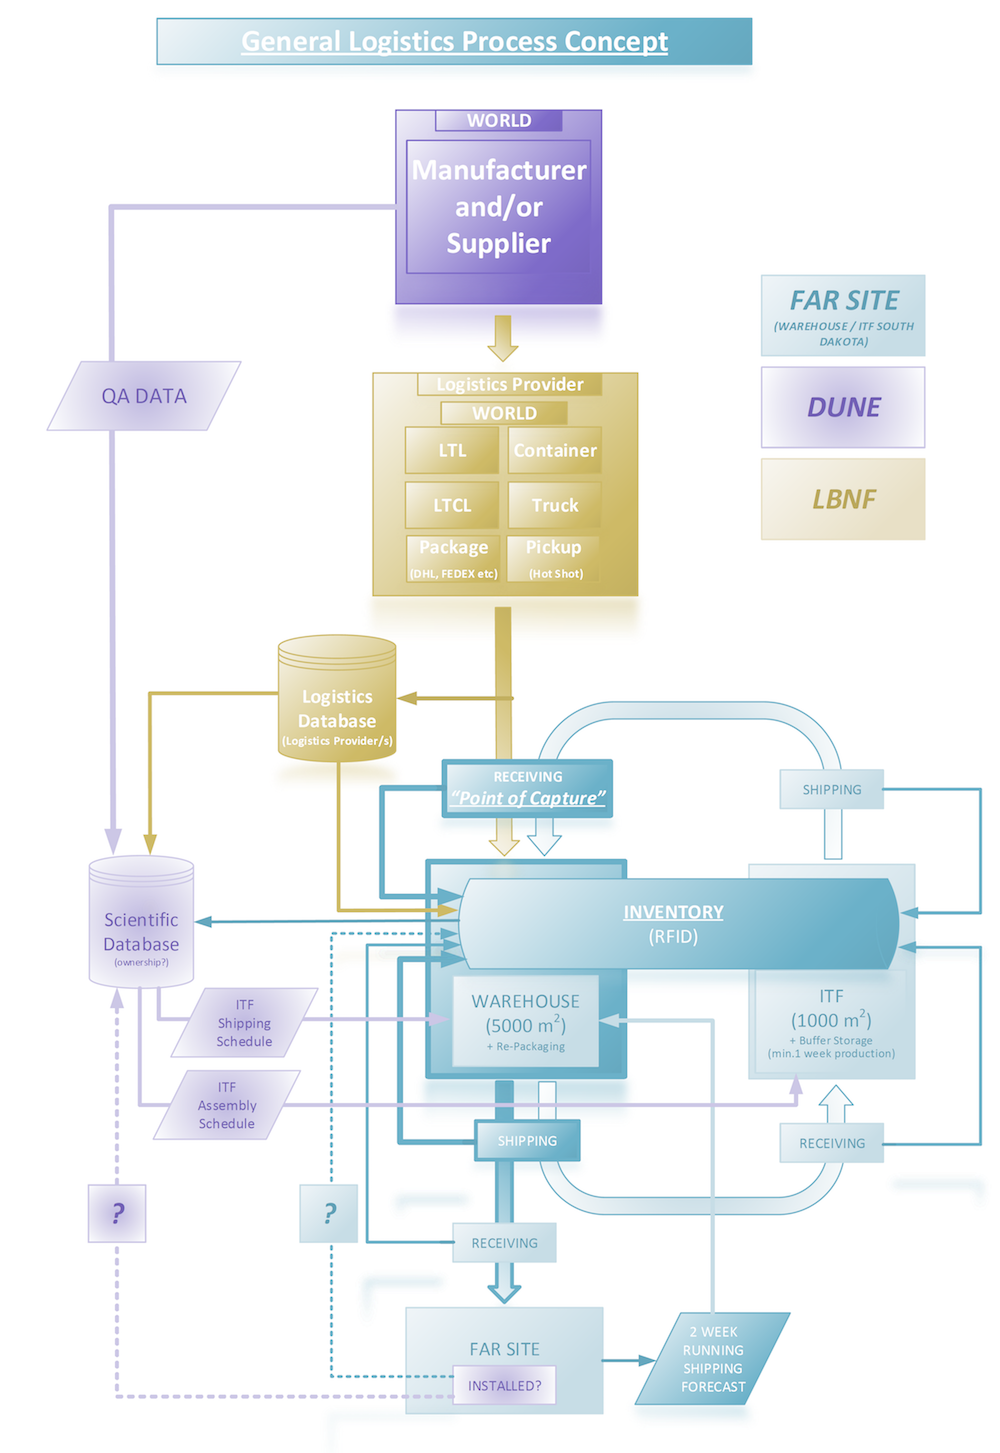
\includegraphics[width=0.85\textwidth]{logistics.png}
\end{dunefigure}

During installation, the height of the Detector Support System beams
is set in accordance to this relationship. Adjustments are done in the
Detector Support System to establish all the beams to be in the
correct plane. The combined effects of gravity prior to fill and
buoyancy after the fill are calculated and further adjustment are made
to compensate. This will ensure that the detector is as close as
possible to design value after fill.

The transverse position of the detector is constrained to be in the
center of the cryostat. As such the mid-plane of the middle row Anode
Plane Assemblies is coplanar with the vertical mid-plane of the
cryostat. This relationship is verified during installation of the
Detector Support System beams and central row of Anode Plane
Assemblies. The outer rows are similarly aligned and surveyed with the
offset as shown in Fig~\ref{fig:dss_feedthru}.
\begin{dunefigure}[Position of feedthrough determining the longitudinal reference point of the detector]{fig:dss_feedthru}
  {Position of feedthrough determining the longitudinal reference point of the detector.}
%  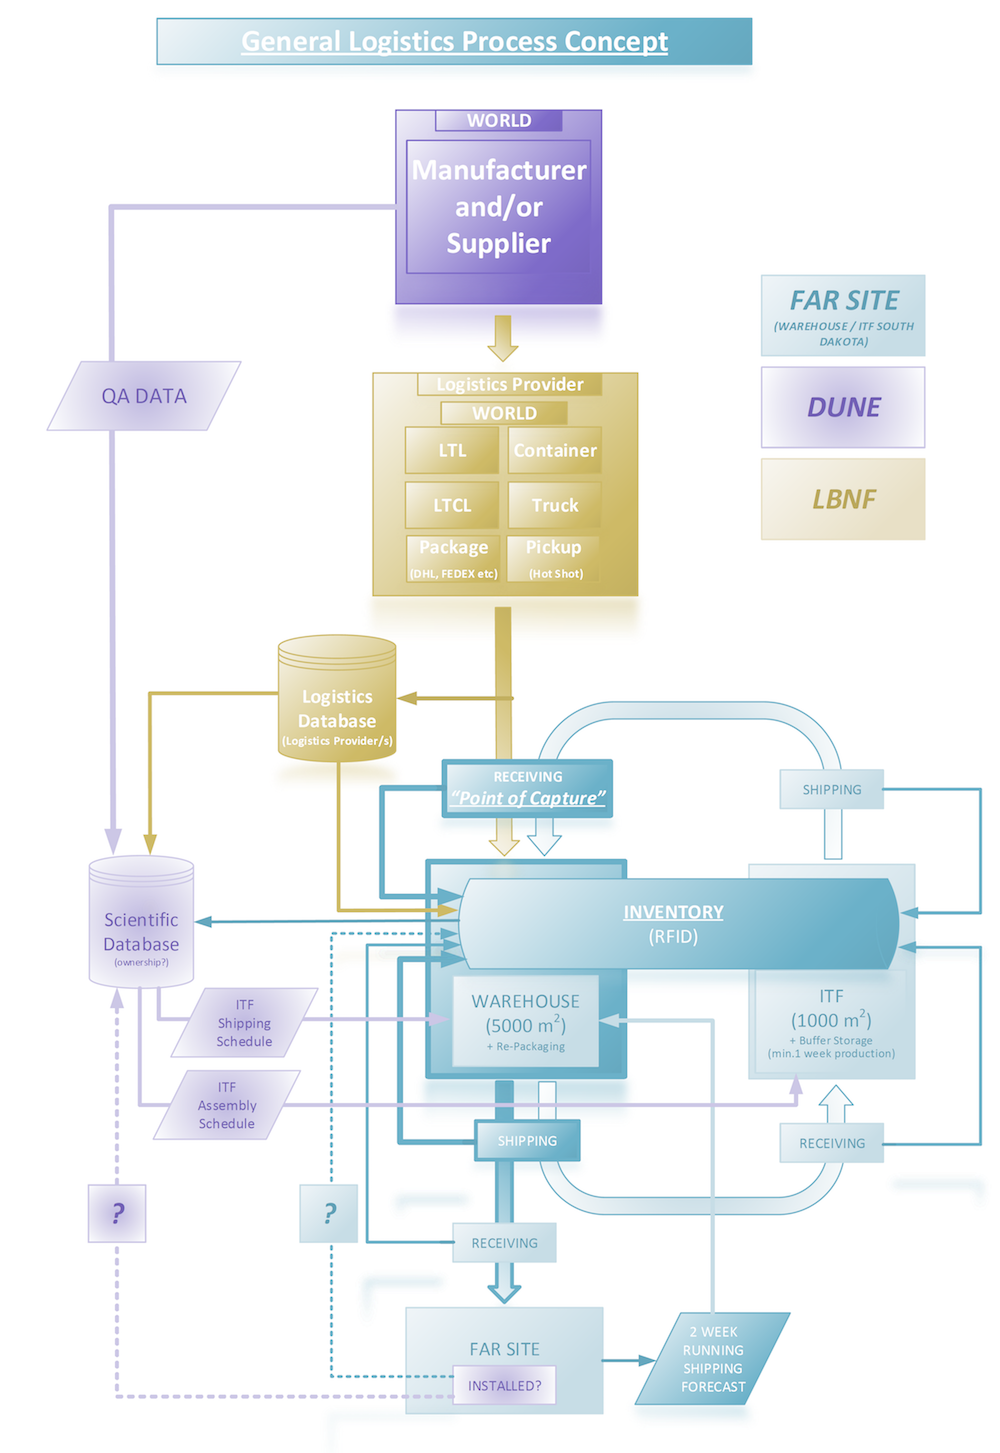
\includegraphics[width=0.85\textwidth]{logistics.png}
\end{dunefigure}


The longitudinal reference point of the detector within the cryostat
is defined by the position of single feedthrough of the central row
that is farthest from the cryostat opening. This feedthrough position
is shown in Fig~\ref{fig:dss_feedthru}.

(Note: The longitudinal position is not fixed at this time. Edit
section as needed once fixed)

(Note: Dual phase be similar
transversely and longitudinally, vertically, it needs to be
determined)


\section{Interface Documents}
\label{sec:fdsp-coord-integ-interface}
Need to write [Farshid/Terri]

consortia-consortia, TC-consortia, TC-LBNF



